\section{Wykorzystanie biblioteki OpenCV}\label{sec:opencv}
Biblioteka OpenCV to otwarte oprogramowanie, które jest wykorzystywane do przetwarzania zdjęć. Jest to narzędzie wspierane przez Windows, Linux, Mac OS oraz Android. W naszej pracy biblioteka została wykorzystana na systemie Ubuntu jednej z wielu dystrybucji systemu Linux w celu wytrenowania własnej kaskady oraz testowania a także na platformie Android by wykorzystać wytrenowane modele zaraz po wykonaniu zdjęcia aparatem. Źródła biblioteki są publicznie dostępne w zdalnym repozytorium \cite{OpenCVSource}. Narzędzia OpenCV umożliwiają wykorzystanie standardu OpenCL który pozwala na równoległe obliczenia z użyciem procesorów centralnych oraz graficznych.


\subsection{OpenCV w procesie trenowania kaskad}

OpenCV oprócz zestawu funkcji operacji na obrazach dostarcza także aplikację pozwalającą na wytrenowanie własnej kaskady cech Haar’a jest to opencv\_traincascade oraz kilka aplikacji które wspierają ten proces to takie aplikacje jak opencv\_createsamples który pozwala stworzyć zbiór uczący na podstawie pojedynczego pozytywnego zdjęcia, opencv\_visualisation umożliwia wizualizację cech włączonych do kaskady w odniesieniu do podanego zdjęcia ze wzorem obiektu którego detekcji uczymy.

\subsubsection{Generowanie zbioru zdjęć pozytywnych}\label{sec:generowanieZdjec}
Przed rozpoczęciem trenowania naszej kaskady klasyfikatorów potrzebne są zdjęcia na których umieszczony jest  obiekt który ma być rozpoznawany oraz kolekcje zdjęć na których nie ma naszego wzorca. By kaskada została skutecznie wytrenowana potrzebne jest jak najwięcej zdjęć. Do wytrenowania kaskady, która rozpoznaje twarze, dołączonej wraz z biblioteką OpenCV wykorzystano 3000 zdjęć pozytywnych oraz 1500 zdjęć negatywnych. Jasnym problemem staje się wykonać taką liczbę zdjęć na którym znajduje się wybrany obiekt a następnie oznaczyć dokładnie jego położenie. Do stworzenia zbioru zdjęć pozytywnych wykorzystano aplikacje opencv\_createsaples. Program ten pozwala na wygenerowania zbioru zdjęć pozytywnych na podstawie jednego zdjęcia na którym tylko i wyłącznie znajduje się przedmiot który potem będzie szukany. Zdjęcie to zostaje wklejane w zbiór zdjęć w losowych miejscach o losowym rozmiarze i o losowym przesunięciu w każdej z trzech płaszczyzn. Dobór zdjęć nie jest dowolny, ważne aby na zdjęciach na które zostanie nałożony nasz obiekt nie był on już umieszczony. Ostatnim elementem potrzebnym do skorzystania z aplikacji opencv\_createsamples jest przygotowanie pliku tekstowego w którym wylistowane będą ścieżki do plików na które mają zostać naniesione wzory naszego obiektu. Dla tak przygotowanych danych możemy uruchomić aplikacje opencv\_createsamples wraz ze wskazanymi parametrami:
\begin{itemize}
    \item -img \textless ścieżka do wzorcowego zdjęcia \textgreater
    \item -bt \textless ścieżka do pliku z opisem zdjęć tła\textgreater
    \item -info \textless ścieżka do pliku w którym mają być zapisane informacje o utworzonych zdjęciach\textgreater
    \item -pngout \textless ścieżka do katalogu w jakim mają być zapisywane pozytywne zdjęcia\textgreater
    \item -bgcolor \textless ośmiobitowa wartośćkoloru tła\textgreater
    \item -bgtrash \textless zakres wartości koloru\textgreater
    \item -maxxangle \textless maksymalny kąt w płaszczyźnie x wyrażony w radianach\textgreater
    \item -maxyangle \textless maksymalny kąt w płaszczyźnie y wyrażony w radianach\textgreater
    \item -maxzangle \textless maksymalny kąt w płaszczyźnie z wyrażony w radianach\textgreater
    \item -num \textless liczba zdjęć która ma zostać wygenerowana>

\end{itemize}

Po uruchomieniu aplikacji we wskazanym folderze zostaną wygenerowane pozytywne zdjęcia 

\begin{figure}[H]
\centering
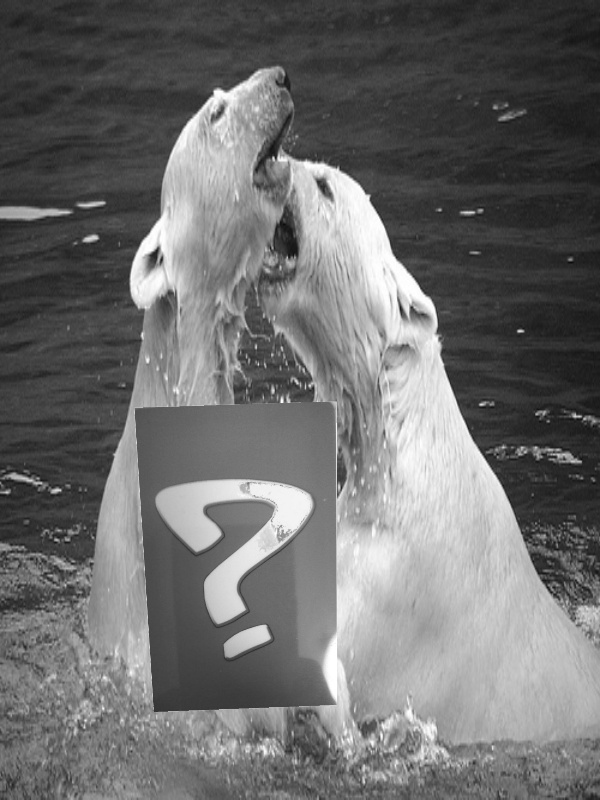
\includegraphics[scale=0.2]{imgs/0448_0134_0398_0203_0316.png}
\caption{Wygenerowane pozytywne zdjęcie}\label{misie}
\end{figure}

Rysunek \ref{misie} przedstawia przykładowo wygenerowane pozytywne zdjęcie. Informacje na temat zdjęcia zapisane we wskazanym pliku info dla tego zdjęcia wygląda następująco
0185\_0196\_0219\_0293\_0454.jpg 1 196 219 293 454
Elementy kolejno oznaczają:

\begin{itemize}
    \item Nazwa pliku
    \item Liczba obiektów na zdjęciu
    \item Współrzędna x lewego górnego rogu obiektu na zdjęciu
    \item Współrzędna y lewego górnego rogu obiektu na zdjęciu
    \item Szerokość obiektu
    \item Wysokość obiektu

\end{itemize}

Posiadając plik info z informacjami na temat położenia zdjęć możemy uzyskać plik z rozszerzeniem vec, który następnie będzie używany przez aplikacje trenującą kaskadę. Posłuży nam do tego także aplikacja opencv\_createsamples. Tym razem należy wskazać następujące parametry:

\begin{itemize}
    \item -info \textless sciezka do pliku info w którym znajdują się informacje o obiektach \textgreater
    \item -vec \textless ściezka do pliku w jakim ma być zapisany plik vec\textgreater
    \item -num \textless ilość zdjęć jaka ma być zapisana w pliku vec\textgreater
    \item -w \textless zerokość obiektu\textgreater
    \item -h \textless wysokość obiektu\textgreater

\end{itemize}

\subsubsection{Trening kaskady}

Do treningu kaskady wykorzystujemy aplikacje opencv\_traincasscade, która implementuje algorytm opisany w punkcie 3.3 . Aplikacja zostanie uruchomiona z następującymi parametrami:

\begin{itemize}
    \item -vec \textless ścieżka do pliku z wektorem opisującym pozytywne zdjęcia \textgreater
    \item -bg \textless sciezka do pliku z zapisanymi ścieżkami plików tworzących zbiór zdjęć negatywnych \textgreater
    \item -numPos \textless liczba pozytywnych zdjęć użyta do treningu \textgreater
    \item -numNeg \textless liczba zdjęć negatywnych użytych do treningu \textgreater
    \item -w \textless szerokość obiektu, taka sama jak w podanym pliku vec \textgreater
    \item -h \textless wysokość obiektu, taka sama jak w podanym pliku vec \textgreater
    \item -numStages \textless liczba elementów z których ma się składać kaskada \textgreater
    \item -maxyangle \textless maksymalny kąt w płaszczyźnie y wyrażony w radianach\textgreater
    \item -maxzangle \textless maksymalny kąt w płaszczyźnie z wyrażony w radianach\textgreater
    \item -num \textless liczba zdjęć która ma zostać wygenerowana>

\end{itemize}

Te parametry są niezbędne do uruchomienia treningu za pomocą tej aplikacji. Możliwe do podania są także inne parametry, które deklarują inną dokładność słabych i silnych klasyfikatorów niż zdefiniowanych domyślnie przez aplikacje. W przypadku podania parametrów które stwierdzają większość dokładność algorytm prawdopodobnie będzie bardziej skuteczny lecz trening będzie trwał dłużej. Natomiast przy zmniejszeniu czas treningu ulegnie skróceniu. Te parametry to:
 
\begin{itemize}
    \item -minHitRate \textless minimalna wartość współczynnika oznaczającego pozytywne klasyfikacje \textgreater
    \item -maxfalsealarm \textless maksymalna dopuszczalna wartość błędnych decyzji \textgreater

\end{itemize}

Podczas trenowania kaskady przydatna jest także aplikacja opencv\_visualisation, która da dotychczasowych etapów generuje podgląd dobranych cech na tle obiektu. Program ten przyjmuje następujące parametry:

\begin{itemize}
    \item -data \textless ścieżka do wygenerowanych obrazów z naniesionymi cechami \textgreater
    \item -image \textless zdjęcie obiektu o rozmiarze takim jaki podany do uczenia kaskady \textgreater
    \item -model  \textless ścieżka do pliku xml z wytrenowanym dotychczas modelem kaskady \textgreater

\end{itemize}

Po uruchomieniu aplikacji zostaną wygenerowane pliki zdjęciowe, osobno dla każdego etapu kaskady. Na każdym z utworzonych obrazów znajduje wizualizacja osobno wszystkich cech wchodzących w skład danego etapu. Obok zdjęć generowany jest także plik wideo w formacie avi na którym przedstawione są po kolei wszystkie cechy wchodzące w skład kaskady na tle obiektu

\begin{figure}[H]
\centering
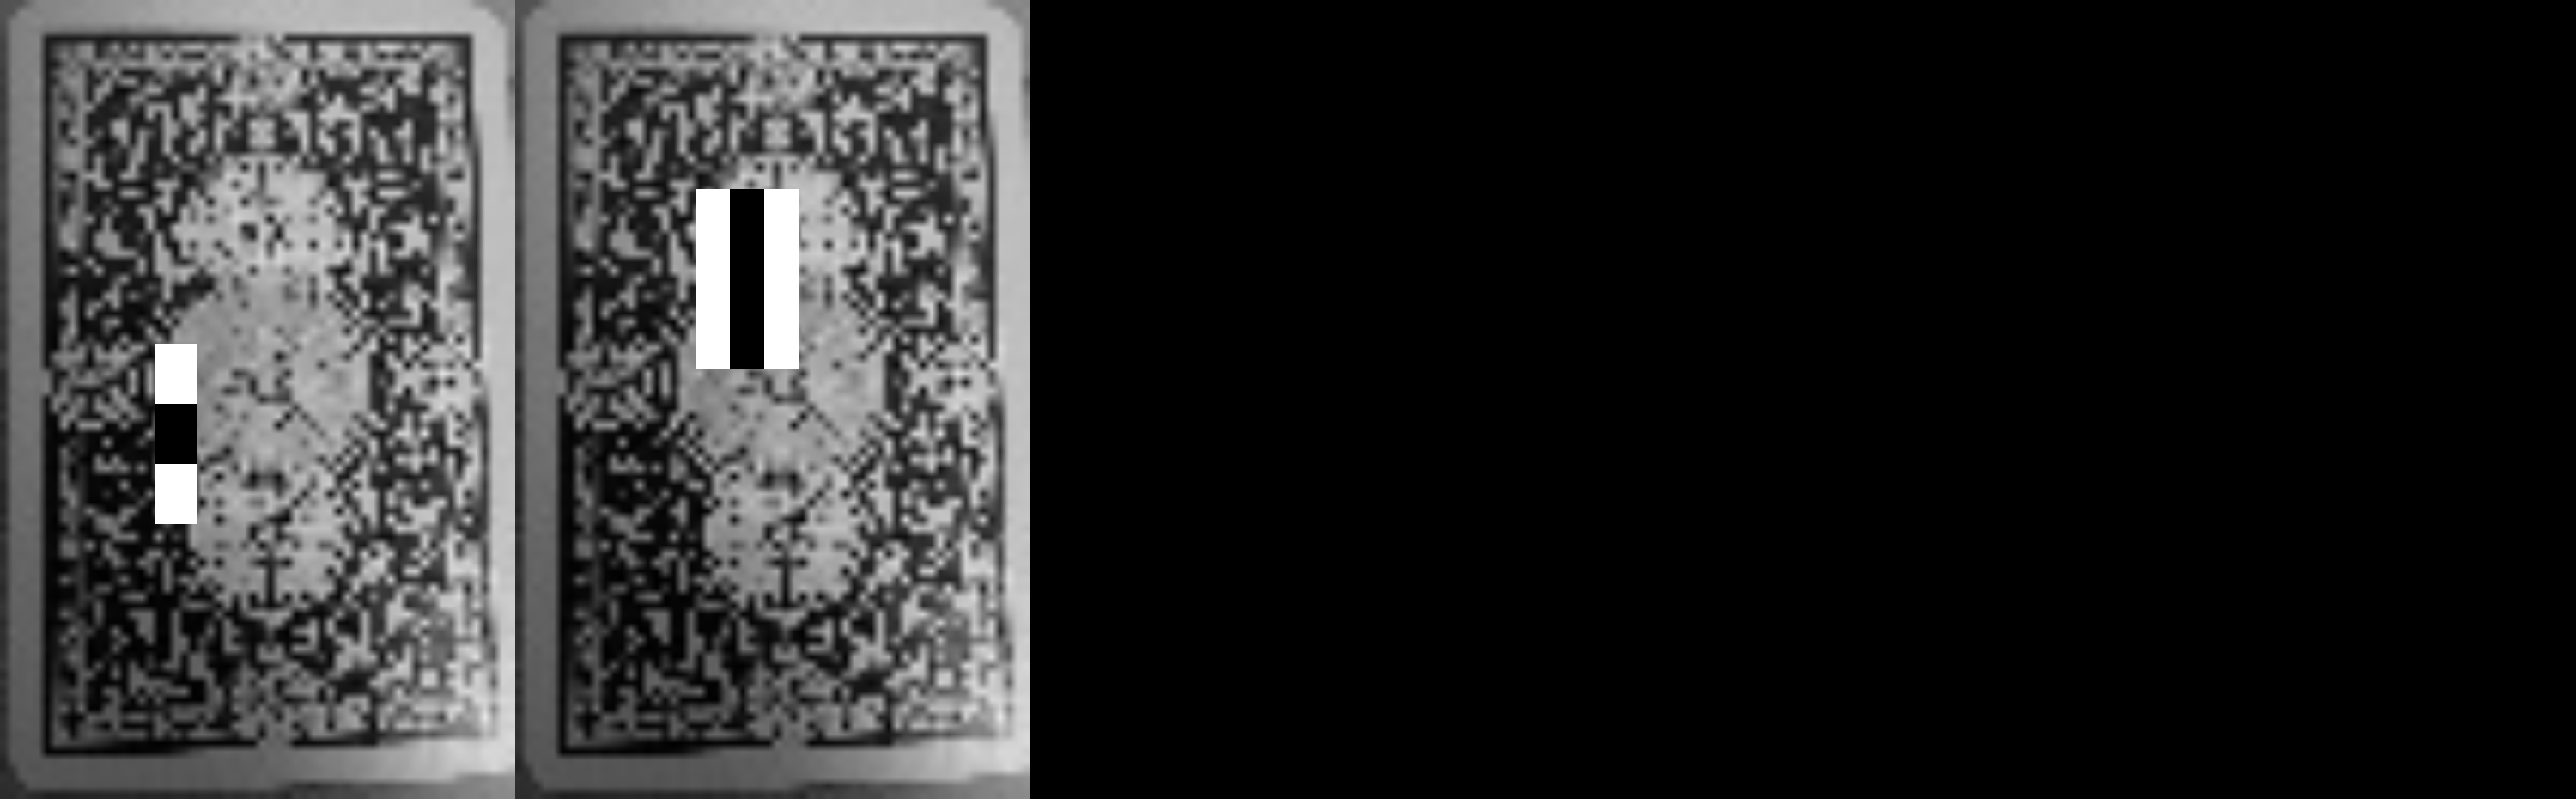
\includegraphics[scale=0.1]{imgs/data3stage_1.png}
\caption{Cechy mocnego asyfikatora}
\end{figure}

\subsection{OpenCV na platformie Android}

Biblioteka OpenCV dla Androida dostarczona jest w zestawie narzędzi deweloperskich OpenCV. Daje ona api Javy. Posiada on prawie wszystkie funkcjonalności Javy. Wszystkie operacje wykonywane są przy użyciu natywnych metod zaimplementowanych w języku C++. Istnieją dwa podejścia w wykorzystaniu tej biblioteki pierwsze zakłada wołanie funkcji poprzez dostarczone api Javy pozwalające bezpośrednio i w łatwy sposób wykorzystanie funkcji w celu przetwarzania obrazu. Wadą takiego podejścia jest wykorzystanie metod JNI, które trwają stosunkowo długo, do tego dochodzi kwestia kopiowania i mapowania obiektów co także mocno wykorzystuje zasoby. Drugie podejście zakłada użycie metod biblioteki z poziomu funkcji natywnych. Zastosowanie takiego rozwiązania jest korzystne jeśli w konkretnym bloku wykonujemy szereg funkcji które z poziomu kodu java wołały by także metody jni. W tym wypadku tak wołana metoda byłaby tylko raz a reszta funkcji wołana by była juz z niskiego poziomu. Takie rozwiązanie jest szybsze oraz wykorzystuje mniej zasobów. Dodatkowo w przypadku wywoływania metod z niskiego poziomu mamy dostęp do 100\% funkcji dostarczanych przez bibliotekę. Jest to rozwiązanie bardziej skomplikowane, trzeba także pamiętać o odpowiednim zarządzaniu pamięcią, gdyż garbage collector działa tylko w ramach maszyny wirtualnej java.

\subsubsection{Detekcja obiektów}

Cały proces detekcji odbywa się przy użyciu kilku funkcji z biblioteki openCV. Na początku należy wczytać zdjęcie. W zależności od źródła zdjęcia może być ono odczytane np jako pojedyncza klatka z kamery lub tak jak w naszym przypadku weźmiemy pojedyncze zdjęcie z pamięci urządzenia. Służy do tego metoda imread wywoływana na obiekcie Imgcodecs. Parametrami tej funkcji są ścieżka do pliku zdjęciowego oraz parametr oznaczający format w jakim ma byc odczytane zdjęcie takimi formatami są:
\begin{itemize}
    \item CV\_LOAD\_IMAGE\_UNCHANGED (\textless0) ładuje zdjęcie w takim formacie w jakim oryginalnie jest zapisane.
    \item CV\_LOAD\_IMAGE\_GRAYSCALE ( 0) ładuję zdjęcie w skali szarości
    \item CV\_LOAD\_IMAGE\_COLOR (\textgreater0) ładuję zdjęcie w formacie BGR
\end{itemize}
Do późniejszej detekcji potrzebujemy zdjęcie wczytane w skali szarości dlatego wczytujemy z parametrem cv2.IMREAD\_GRAYSCALE.
Załadowane zdjęcie znajduje się w obiekcie klasy Mat. Jest to klasa przechowująca macierze oraz obrazy. Posiada wiele właściwości opisujące zdjęcie takie jak np rozmiar.
Do detekcji potrzebujemy załadować także nasz plik z kaskadą w formacie xml. Tworzymy obiekt klasy CascadeClassifier, w konstruktorze obiektu podajemy ścieżkę do naszego wytrenowanego modelu. Kiedy mamy przygotowany obraz oraz kaskadę możemy na kaskadzie zawołać metodę detectMultiScale która w parametrach przyjmuje obiekt Mat w którym znajduje się załadowane zdjęcie na którym szukamy obiektu, referencja do kolekcji MatOfRect do którego zostaną zapisane fragmenty zdjęcia z szukanym obiektem, scaleFactor to następny parametr, który określa zmianę wielkość przeszukiwanego fragmentu w kolejnych iteracjach algorytmu. Wysoka wartość tego parametru sprawia, że różnica między klasyfikatorami w kolejnych iteracjach jest większa. Mała wartość parametru sprawia, że większa ilość fragmentów zostanie przeszukana co sprawia, że detekcja trwa długo. Wysoka wartość przyspiesza znacząco czas działania algorytmu lecz istnieje możliwość pominięcia przeoczenia szukanego elementu. Kolejny parametr to minNeighbors który określa minimalną ilość sąsiednich fragmentów uznanych jako wykryty obiekt, żeby uznać go za pozytywny. Kolejne parametry to obiekty typu size określające minimalną wielkość i maksymalną wielkość szukanego obiektu. Jeśli różnica tych wielkości jest duża czas algorytmy się wydłuży gdyż więcej różnych wielkości będzie musiało zostać sprawdzonych. 
Po wykonaniu metody detectMultiScale kolekcji MatOfRect zapisane są informacje o współrzędnych odnalezionych obiektów,w tych miejscach możemy wkleić prostokąt lub w jakiś inny sposób modyfikować.
